\documentclass[14pt]{extarticle}
\usepackage{amsmath}
\usepackage{amssymb}
%\usepackage{tikz}
%\usetikzlibrary{calc}
%\usetikzlibrary{trees}
\usepackage{hyperref}
\usepackage{graphicx}
\graphicspath{ {../../chap11/} }
\usepackage[top=0.75in, bottom=0.75in, left=0.75in, right=0.75in]{geometry}
%\newcommand*{\Scale}[2][4]{\scalebox{#1}{\ensuremath{#2}}}%
\usepackage[shortlabels]{enumitem}
\usepackage[most]{tcolorbox}
\definecolor{bg}{RGB}{255,249,227}
% \usepackage{showframe}

\title{\vspace{-5ex}Math 208 Section 11.2}
\date{\vspace{-10ex}}
\usepackage{multicol}
\setlength{\columnsep}{1cm}
\setlength{\parindent}{0pt}
\usepackage{parskip}
\setlength{\parskip}{10pt} % 1ex plus 0.5ex minus 0.2ex}
%\usepackage{ragged2e}



\begin{document}
	\maketitle
	
\section{Homework, Reading, and Other}
\begin{itemize}
	\item Section 11.1
	\item Section 11.2
\end{itemize}

\section{Goals}
\begin{itemize}
	\item Understand what the second derivative tells us about the graph of a function
	\item Create and interpret a sign chart
	\item Draw graphs using the sign chart
\end{itemize}


\section{Section 11.2: Second Derivative and Graphs}
What is a \textit{second derivative} of a function? It is simply the derivative of the first derivative of the function. The second derivative of $f(x)$ is denoted by $f''(x)$. If you know how to find the derivative of a function, you know how to find the second derivative.

\subsection{Introduction}
What is the difference between the two graphs shown below?
\begin{center}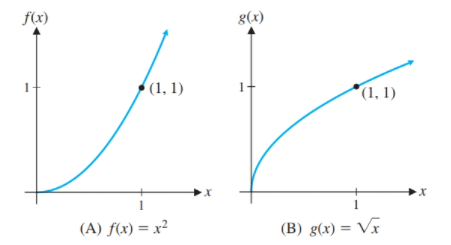
\includegraphics[width=0.7\linewidth]{11-2-a1}\end{center}
Obviously, the first curves up and the second curves down. We call this concavity. But what tools do we already have that helps us determine this behavior in a function?

Not much? Let's consider this more deeply. We can say that the slope of the tangent lines in graph (A) are increasing while those in graph (B) are decreasing.

Let's summarize some information about (A), i.e. $f(x)$.
\begin{itemize}
	\item $f$ is an increasing function that is concave upward.
	\item Since $f$ is increasing, $f'$ is always positive.
	\item Since the slope of the tangent line is increasing, we can say that $f'$ is increasing. Considering $f'$ as a function, this is equivalent to stating that the derivative of $f'$ is positive. This is $f''$! So we have that $\mathbf{f''}$ \textbf{is positive}.
\end{itemize}

Let's summarize some information about (B), i.e. $g(x)$.
\begin{itemize}
	\item $g$ is an increasing function that is concave downward.
	\item Since $g$ is increasing, $g'$ is always positive.
	\item Since the slope of the tangent line is increasing, $\mathbf{g''}$ \textbf{is negative}.
\end{itemize}

\subsection{Second Derivative}
\begin{tcolorbox}[enhanced jigsaw,colback=bg,boxrule=0pt,arc=0pt]
	\textbf{Second Derivative} \\
	For $y=f(x)$, the second derivative of $f$, if it exists, has these various notations:
	$$f''(x) = \frac{d}{dx}f'(x)=\frac{d^2y}{dx^2}=y''$$
\end{tcolorbox}

\subsubsection{Examples}
\begin{enumerate}
	\item Find the second derivative of $f(x) = x^2$
	\begin{align*}
		f(x) &= x^2 \\
		f'(x) &= 2x \\
		f''(x) &= 2
	\end{align*}
	Notice that $f''$ is a positive constant. This matches our result for graph (A).
	\item Find the second derivative of $g(x) = \sqrt{x}$
	\begin{align*}
		g(x) &= x^{1/2} \\
		g'(x) &= \frac{1}{2}x^{-1/2} \\
		g''(x) &= -\frac{1}{4}x^{-3/2} =  -\frac{1}{4\sqrt{x^3}}
	\end{align*}
	Notice that for all $x<0$, $g''$ is a negative. This matches our result for graph (B).
\end{enumerate}


\subsection{Understanding the graph and second derivative}
The second derivative informs us about the concavity of the graph.
 \begin{center}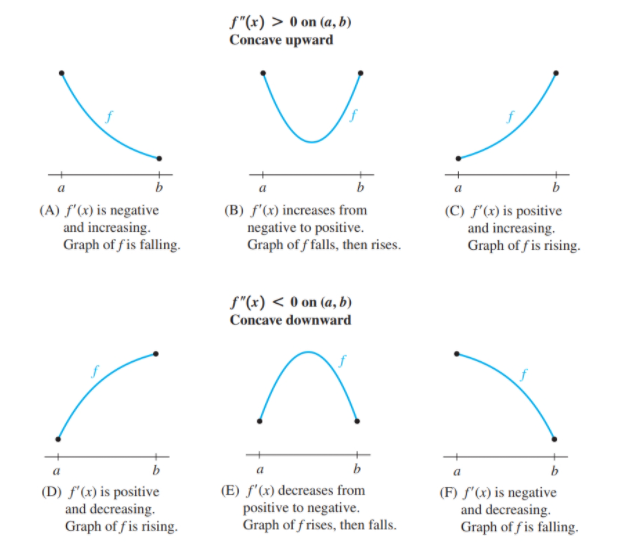
\includegraphics[width=1\linewidth]{11-2-1}\end{center}
\vspace{1em}

What about when $f''=0$ or is not defined? Well, then we have an inflection point on the graph. We will now be adding the second derivative to our sign charts.
\begin{center}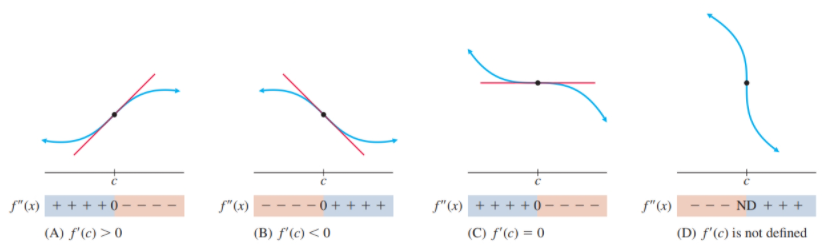
\includegraphics[width=1\linewidth]{11-2-2}\end{center}

\subsubsection{Examples of Finding Inflection Points}
Find the intervals on which the graph of f is concave upward, the intervals on which the graph of f is concave downward, and the x, y coordinates of the inflection points.

\textbf{Ex1} (32)  $f(x) = 3x^4 -18x^2$.

Start by finding the partition points of $f''$ to determine the intervals. Then use test points to determine concavity.
\begin{align*}
	f(x) &= 3x^4 -18x^2 \\
	f'(x) &=12x^3-36x \\
	f''(x) &= 36x^2-36 &\text{Set equal to 0}\\
	&36x^2-36 = 0 \\
	&x^2 = 36/36 = 1
\end{align*}
So the partition points of $f''$ are $x=-1$ and $x=1$. Use test points $-2, 0, 2$
\begin{align*}
	f''(-2) &= 108 \\
	f''(0) &= -36 \\
	f''(2) &= 108
\end{align*}
The values of y at the critical points are: $f(-1) = -15$ and $f(1) = -15$. The y-intercept is $f(0)=0$. The sign chart is
\begin{verbatim}
  x    |      -1     0       1
f(x)   |     -15     0     -15  
f''(x) | +++   0 ---   ---   0  +++         
\end{verbatim}
From this we have
\begin{itemize}
	\item $(-\infty, -1)$ is concave upward
	\item $(-1,1)$ is concave downward
	\item $(1,\infty)$ is concave upward
\end{itemize}
\vspace{1em}


\textbf{Ex2} (36)  $f(x) = x^4 -2x^3-5x+3$.

Start by finding the partition points of $f''$ to determine the intervals. Then use test points to determine concavity.
\begin{align*}
	f(x) &= x^4 -2x^3-5x+3 \\
	f'(x) &= 4x^3-6x^2-5 \\
	f''(x) &= 12x^2 -12x &\text{Set equal to 0}\\
	&12x(x -1) = 0
\end{align*}
So the partition points of $f''$ are $x=0$ and $x=1$. Use test points $-1, 1/2, 2$
\begin{align*}
	f''(-1) &= 24 \\
	f''(1/2) &= -3\\
	f''(2) &= 24
\end{align*}
The values of y at the critical points are: $f(0) = 3$ and $f(1) = -3$. The y-intercept is $f(0)=3$. The sign chart is
\begin{verbatim}
	x      |     0      1      
	f(x)   |     3     -3
	f''(x) | +++ 0 ---  0 +++      
\end{verbatim}
From this we have
\begin{itemize}
	\item $(-\infty, -1)$ is concave upward
	\item $(-1,1)$ is concave downward
	\item $(1,\infty)$ is concave upward
\end{itemize}

\subsection{Curve Sketching}
Calculators and computers do a great job of plotting graphs, but they do this by literally plotting points without care for the importance of critical points. In our analysis, we are offten concerned with these critical points and these points also make it reasonable to sketch the curve.

\begin{center}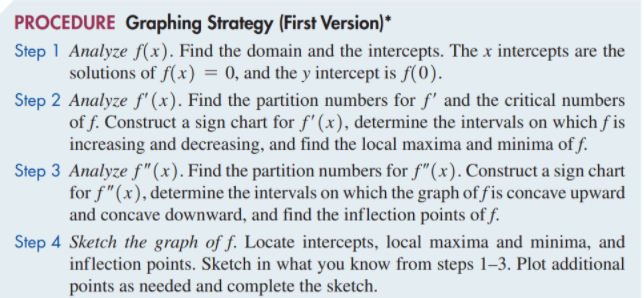
\includegraphics[width=1\linewidth]{11-2-3}\end{center}

\subsubsection{Curve Sketching Examples} Use the Graphing Strategy then sketch the graph.
\begin{enumerate}
	\item (Matched Problem 5)  $f(x)=x^4+4x^3$.
	
	\textbf{Step 1:} The domain of $f(x)$ is all $x$.
	\begin{align*}
		f(x) &=x^4+4x^3 =0 \\
		&x^3(x+4) = 0 \\
		\text{When } &x=-4\\
		&x=0 \\\\
		f(0) &=0
	\end{align*}

	\textbf{Step 2:}
	\begin{align*}
		f'(x) &=4x^3+12x^2 = 0 \\
		&4x^2(x+3)	=0 \\
		\text{When } &x=-3\\
		&x=0 \\\\
		f(-3) &= -27
	\end{align*}
	Test points are, $x=-4, x=-1$, and $x=1$
	\begin{align*}	
		f'(-4) &= -64 \\
		f'(-1) &=8 \\
		f'(1) &= 16
	\end{align*}

	\textbf{Step 3:}
	\begin{align*}
		f''(x) &= 12x^2 + 24x =0 \\
		&12x(x+2) = 0 \\
		\text{When } &x=-2\\
		&x=0 \\\\
		f(-2) &= -16
	\end{align*}
	Test points are, $x=-4, x=-1$, and $x=1$
	\begin{align*}	
		f''(-4) &= 96 \\
		f''(-1) &=-12 \\
		f''(1) &= 36
	\end{align*}
	
\begin{verbatim}
  x    |     -4    -3      -2     0    
f(x)   |      0   -27     -16     0  
f'(x)  |       ---  0 +++         0 +++
f''(x) |             +++    0 --- 0 +++
\end{verbatim}

\textbf{Step 4:} Sketch the curve.

\vspace{2em}

\item (Matched Problem 6)  $f(x)=3x^{2/3}-x$.

\textbf{Step 1:} The domain of $f(x)$ is all $x$.
\begin{align*}
	f(x) &=3x^{2/3}-x =0 \\
	&3x(\frac{1}{\sqrt[3]{x}}-\frac{1}{3}) = 0 \\
	\text{When } &x=0\\
	&x=27 &\text{ Since $\sqrt[3]{27}=3$} \\\\
	f(0) &=0
\end{align*}

\textbf{Step 2:}
\begin{align*}
	f'(x) &= 2x^{-1/3} -1 = 0 \\
	&\frac{1}{\sqrt[3]{x}}	=1/2 \\
	\text{When } &x=8 \\
	\text{Also ND when } &x=0\\\\
	f(8) &= 4
\end{align*}
Test points are, $x=-1, x=1$, and $x=27$
\begin{align*}	
	f'(-1) &= -3 \\
	f'(1) &=1 \\
	f'(27) &= -1/3
\end{align*}

\textbf{Step 3:}
\begin{align*}
	f''(x) &= -\frac{2}{3}x^{-4/3} =0 \\
	\text{ND when } &x=0
\end{align*}
Test points are, $x=-1$, and $x=1$
\begin{align*}	
	f''(-1) &= -2/3 \\
	f''(1) &= -2/3
\end{align*}

\begin{verbatim}
	x      |      0     8    27    
	f(x)   |      0     4     0
	f'(x)  | --- ND +++ 0 ---  
	f''(x) | --- ND ---   
\end{verbatim}

\textbf{Step 4:} Sketch the curve.
	
\end{enumerate}

Typically, you will be working with whole exponent polynomials. Like example 1.


\noindent\rule{\textwidth}{1pt}
{\footnotesize Copyright (C) 2021 Garold Dalton --- Released under GNU General Public License v3.0}


\cleardoublepage	
	
\end{document}
